\documentclass[../main.tex]{subfiles}
%!TEX root = ./analysisThrusterArms.tex
\graphicspath {{../}}

\begin{document}
\subsection{Thruster Arms} \label{thrustArms}

\begin{figure}[H]
	\centering
	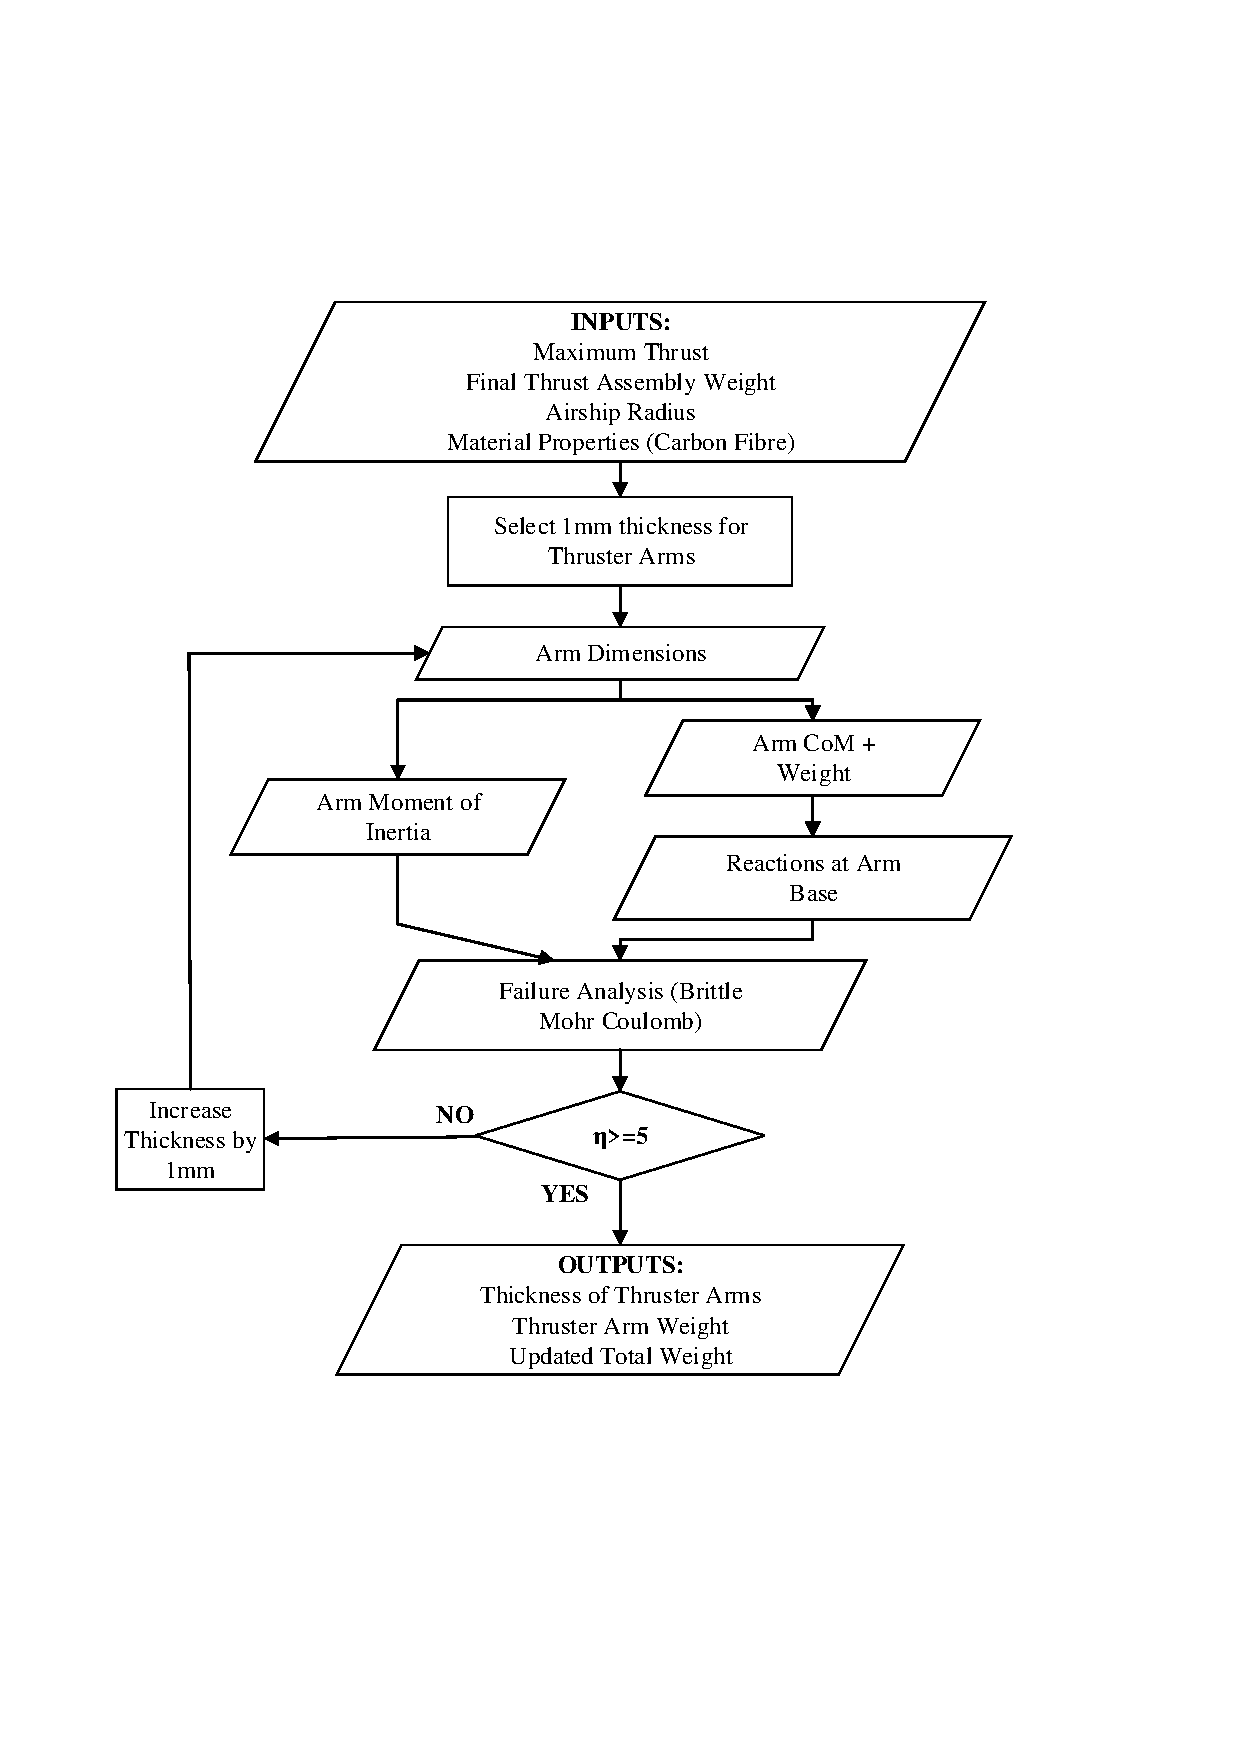
\includegraphics[width=.9\linewidth]{img/paramaterization/thrusterArms.pdf}
	\caption{Parametrization Outline for the Thruster Arms}
	\label{fig:thrusterArmsParametrization}
\end{figure}

The thruster arm analysis is preformed to determine the required arm thickness to meet the specified safety factor. The analysis will also out put the weight of the arms and re compute the weight of the entire thruster assembly and its center of gravity data. In order to run the analysis several inputs are required including the maximum thrust force, thruster assembly weight, the airship radius, and the material properties of the carbon fiber the arms will be fabricated from. In order to minimizing stress concentrations and increase ease of manufacturing the width of the arms is held constant and 30[mm]. This width enables the arms to remain the same width as the section where the keel connector is inserted as seen in FIG???. 

The scenario for the analysis is that descried in Loading Scenario, Section \ref{loadingScenarios}, Maximum Downward Force show in FIG??? where all forces are with reference to the coordinate system $XYZ$ defined by the pitch of the airship. The analysis begins by computing the reaction forces and moments at the point at the center of the inner radius pf the arms as seen in FIG???. In order to do so the code REF??? sums all the weights of all the thruster assembly components and has them acting at their center of gravity. The following equation \ref{eqn:armCg} is used to solve for the center based on the inner and outer radii $r_o$ and $r_i$. Because of symettry the center of gravity in Z is the same of that in Y but negative. 
\begin{equation} \label{eqn:armCg}
armCg =4(r_o^3 - r_i^3)/(3*pi()*(ro^2 - ri^2));
\end{equation}
 It also considers the maximum thrust force. once the code solves the reaction forces it computes both the 

For this section, the arm will be analyzed with only being supported by the connection to the keel. Each loading scenario will having it's own assumption. The dimensions of the arm can be seen in Figure \ref{fig:ArmDimensions}, which will be used in this section.

Not shown on the figure, but useful for analysis is the two radii for the neutral axis of the curve:
\begin{equation} \label{eqn:CurveRs}
\bar{r} = r_i + \frac{h}{2}, \quad r = \frac{h}{ln(r_o/r_i)}
\end{equation}

%	Z-DIRECTION
\subsubsection{Z-Direction}
For this loading scenario the failure point is assumed to be at or near the location of the reaction forces. The inputs for this analysis come from the Force Calculation Section, which finds the reaction forces. It is assumed that the main failure will come from stress on the inner edge of the curved member. The inner edge being in tension is calculated using:
\begin{equation} \label{eqn:CurveStress}
\sigma _i = \frac{Mc_i}{eAr_i}
\end{equation}
Where $A = hk$, $e = \bar{r} - r$, and $c_i = r - r_i$. The moment force has multiple forces and distances which are found in Figure \ref{fig:ArmThrustDown}, the equal moment acting on each half of the arm can be found:
\begin{equation} \label{eqn:CurveMoment}
M = BW_{S} + CW_E + DW_T + EF_T 
\end{equation}

$W_S$ and $W_E$ are related to the analysis of this component, since the changing dimensions will change the weight, as well as potentially change the centre of mass of the components. To simplify some of the equations the thickness of the arm can be taken as $h = r_o - r_i$. The equations for the weights are s below:
\begin{equation} \label{eqn:CurveSupportWeight}
B= \frac{4(r_o^3-r_i^3)}{3\pi (r_o^2-r_i^2)}, \quad 
W_{S} = \frac{k\pi(r_o^2-r_i^2)}{4}g\rho_{material}
\end{equation}

\begin{equation} \label{eqn:EnvelopeSupportWeight}
C = r_i + h/2, \quad 
W_{E} = \frac{ha(2b-k)}{2}g\rho_{material}
\end{equation}

Solving for the inner stress of the member will give the stress used in the safety factor of the component. This is done using the following equation:
\begin{equation} \label{eqn:CurveSafetyFactor}
\eta = \frac{S_y}{\sigma_i}
\end{equation}

\end{document}